\documentclass[11pt,letterpaper]{article}
\usepackage[utf8]{inputenc}
\usepackage[english]{babel}
\usepackage{titlesec}
%%%%%%%%%%%%%%%%%%%%%%%%%%%%%%%%%%%%%%%%%%%%%%%%%%%%%
\usepackage{amsmath}
\usepackage{amsfonts}
\usepackage{amssymb}
\usepackage{mathtools}
\usepackage[margin=1in]{geometry}
%%%%%%%%%%%%%%%%%%%%%%%%%%%%%%%%%%%%%%%%%%%%%%%%%%%%%
\usepackage{graphicx}
\usepackage{tikz}
\usetikzlibrary{calc}
\usepackage{tikz-3dplot}
%%%%%%%%%%%%%%%%%%%%%%%%%%%%%%%%%%%%%%%%%%%%%%%%%%%%%
\usepackage{varioref}
\usepackage{fancyref}
\usepackage{float}
\floatstyle{boxed}
\restylefloat{figure}
\usepackage{framed}
%%%%%%%%%%%%%%%%%%%%%%%%%%%%%%%%%%%%%%%%%%%%%%%%%%%%%
\usepackage{listings}
\usepackage{color}

\titleformat{\subsection}[runin]
  {\normalfont\large\bfseries}{\thesubsection}{1em}{}
\titleformat{\subsubsection}[runin]
  {\normalfont\normalsize\bfseries}{\thesubsubsection}{1em}{}

\definecolor{dkgreen}{rgb}{0,0.6,0}
\definecolor{gray}{rgb}{0.5,0.5,0.5}
\definecolor{mauve}{rgb}{0.58,0,0.82}

\lstset{language=Java,
  aboveskip=3mm,
  belowskip=3mm,
  showstringspaces=false,
  columns=flexible,
  basicstyle={\small\ttfamily},
  numbers=none,
  numberstyle=\tiny\color{gray},
  keywordstyle=\color{blue},
  commentstyle=\color{dkgreen},
  stringstyle=\color{mauve},
  breaklines=true,
  breakatwhitespace=true,
  tabsize=3
}
%%%%%%%%%%%%%%%%%%%%%%%%%%%%%%%%%%%%%%%%%%%%%%%%%%%%%
%Script R%
\usepackage{calligra}
\usepackage{qtree}
\DeclareMathAlphabet{\mathcalligra}{T1}{calligra}{m}{n}
\DeclareFontShape{T1}{calligra}{m}{n}{<->s*[2.2]callig15}{}
\newcommand{\scripty}[1]{\ensuremath{\mathcalligra{#1}}}
\newcommand{\sr}{\scripty{r}}
\newcommand{\vsr}{\vec{\sr\,}}
%%%%%%%%%%%%%%%%%%%%%%%%%%%%%%%%%%%%%%%%%%%%%%%%%%%%%
%Macros%
\newcommand{\dint}[2]{\int\limits_{#1}^{#2}}

%%%%%%%%%%%%%%%%%%%%%%%%%%%%%%%%%%%%%%%%%%%%%%%%%%%%%
\author{Alex Pizzuto}
\title{CS 367 Homework 5}
\begin{document}
\date{}
\maketitle
\hrule

\section{Question One}
We are given the following shaker sort (bi-directional bubble sort) algorithm:
\begin{lstlisting}
	begin = 0, end = A.length-1

	// At the beginning of every iteration of this loop, we know that the 
	// elements in A are in their final sorted positions from A[0] to A[begin-1]
	// and from A[end+1] to the end of A.  That means that A[begin] to A[end] are
	// still to be sorted.
	do
	    for i going from begin to end-1
	        if A[i] and A[i+1] are out of order, swap them
	    end--

	    if no swaps occurred during the preceding for loop, the sort is done

	    for i going from end to begin+1
	        if A[i] and A[i-1]  are out of order, swap them
	    begin++
	 until no swaps have occurred or begin >= end
\end{lstlisting}
\subsection{A: Best Case Time Complexity}
The best case time complexity is just $O(N)$ where $N$ is the size of the array. This occurs when the values were already in sorted order. In this case, no swaps occur, and the array is only iterated over once, with $O(1)$ comparisons being made $N$ times, resulting in $O(N)$. The sort will then stop as no swaps occurred. 
\subsection{B: Worst Case Time Complexity}
The worst case time complexity for this sort is $O(N^2)$. This occurs when the array is in reverse order. In this case, the maximum number of swaps occurs during each pass forwards and backwards through the array. This means that during the first (forward) iteration, there would be $N$ swaps. Then, backwards, there would be $N-1$ swaps (as now one element is in place). This will keep happening, and the overall complexity is given by 
\begin{equation*}
	\sum_{i=0}^{N}i = 1 + 2 + \cdots + N
\end{equation*}
which we know is bounded by $O(N^2)$.

\section{Question Two}
\subsection{A}
Now, suppose instead of needing to sort an entire array, we need only extract the smallest (or largest) \emph{K} items from the list. If we can only choose between insertion sort and selection sort, then selection sort is easier to modify so that it \textit{efficiently} gives us only the smallest \emph{K} items in sorted order. 
\subsection{B}
In order to make this change, we need to change the algorithm so that the outer loop, instead of iterating from index 0 to index \texttt{length - 1}, we only go from index 0 to index \texttt{K - 1}. 
\subsection{C}
Insertion sort cannot be modified to what we want to do efficiently. We will prove this via counterexample. Take the case where we want the smallest 5 values in the array \texttt{A}. Also suppose that one of these values lies in \texttt{A[length - 1]}. For insertion sort, the entire algorithm needs to operate, and we need to sort all elements in smaller indices before finding this value, so the worst case complexity is the worst case complexity of a full insertion sort, while the worst case for selection sort with modification is $O(N*K)$, where $N$ is the length of the array and $K$ is the number of extremes that we desire. 

\section{Question Three}
Using median-of-three pivot selection, we show the successive changes that are made as quicksort partitions the following list of integers:
\newline

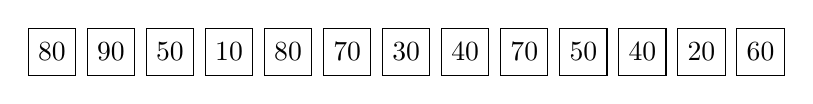
\begin{tikzpicture}
    \coordinate (s) at (0,0);
    \foreach \num in {80,90,50,10,80,70,30,40,70,50,40,20,60}{
      \node[minimum size=6mm, draw, rectangle] at (s) {\num};
      \coordinate (s) at ($(s) + (0.75,0)$);
    }
\end{tikzpicture}

Use median of three pivot selection, move these three items
\newline

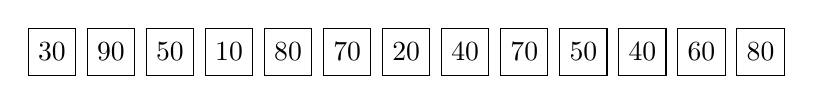
\begin{tikzpicture}
    \coordinate (s) at (0,0);
    \foreach \num in {30,90,50,10,80,70,20,40,70,50,40,60,80}{
      \node[minimum size=6mm, draw, rectangle] at (s) {\num};
      \coordinate (s) at ($(s) + (0.75,0)$);
    }
\end{tikzpicture}

Switch 90 and 40
\newline

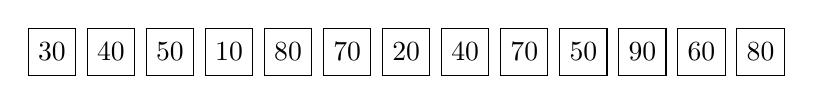
\begin{tikzpicture}
    \coordinate (s) at (0,0);
    \foreach \num in {30,40,50,10,80,70,20,40,70,50,90,60,80}{
      \node[minimum size=6mm, draw, rectangle] at (s) {\num};
      \coordinate (s) at ($(s) + (0.75,0)$);
    }
\end{tikzpicture}

Switch 80 and 50
\newline

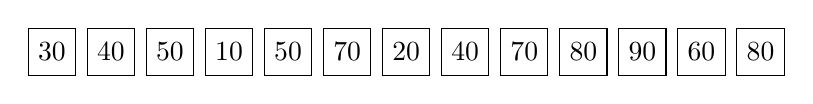
\begin{tikzpicture}
    \coordinate (s) at (0,0);
    \foreach \num in {30,40,50,10,50,70,20,40,70,80,90,60,80}{
      \node[minimum size=6mm, draw, rectangle] at (s) {\num};
      \coordinate (s) at ($(s) + (0.75,0)$);
    }
\end{tikzpicture}

Switch 70 and 40
\newline

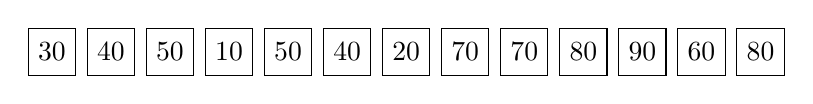
\begin{tikzpicture}
    \coordinate (s) at (0,0);
    \foreach \num in {30,40,50,10,50,40,20,70,70,80,90,60,80}{
      \node[minimum size=6mm, draw, rectangle] at (s) {\num};
      \coordinate (s) at ($(s) + (0.75,0)$);
    }
\end{tikzpicture}

Switch to return pivot
\newline

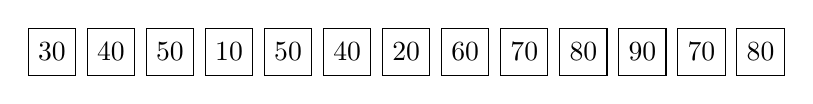
\begin{tikzpicture}
    \coordinate (s) at (0,0);
    \foreach \num in {30,40,50,10,50,40,20,60,70,80,90,70,80}{
      \node[minimum size=6mm, draw, rectangle] at (s) {\num};
      \coordinate (s) at ($(s) + (0.75,0)$);
    }
\end{tikzpicture}





\end{document}